\documentclass{article}

\usepackage[english]{babel}
\usepackage[utf8]{inputenc}
\usepackage{amsmath,amssymb}
\usepackage{parskip}
\usepackage{graphicx}
\usepackage{subfig}
\usepackage{titling}
\usepackage{float}
% Margins
\usepackage[top=2.54cm, left=2.54cm, right=2.54cm, bottom=2.54cm, textheight=11pt]{geometry}

\predate{}
\postdate{}
\title{\vspace{-1.8cm}\textbf{2 Dimensional Unsteady Heat Diffusion}}
\author{Nikhil Thota}
\date{}

\begin{document}
\maketitle

\section{Method and Results}

The 2-D unsteady heat diffusion equation : $ \dfrac{\partial T(i,j)}{\partial t} = \alpha\dfrac{\partial^2 T(i,j)}{\partial x^2} + \alpha\dfrac{\partial^2 T(i,j)}{\partial y^2} $

The finite difference method was used to convert the partial differential equation into a difference equation. $ \dfrac{\partial T(i,j)}{\partial t} $ was converted using \textbf{First-order forward difference} while $\dfrac{\partial^2 T(i,j)}{\partial x^2}$ and $\dfrac{\partial^2 T(i,j)}{\partial y^2}$ were converted to their difference forms using \textbf{Second-order central difference}. This is shown below : 

\textbf{First-order forward difference :} $ \dfrac{\partial T(i,j)}{\partial t} = \dfrac{T^{n+1}(i,j) - T^{n}(i,j)}{\Delta t} $

\textbf{Second-order central difference :}

$$ \dfrac{\partial^2 T(i,j)}{\partial x^2} = \dfrac{T^{n}(i+1,j) - 2T^{n}(i,j) + T^{n}(i-1,j)}{\Delta x^2} $$

$$ \dfrac{\partial^2 T(i,j)}{\partial y^2} = \dfrac{T^{n}(i,j+1) - 2T^{n}(i,j) + T^{n}(i,j-1)}{\Delta y^2} $$



Substituting in the 2-D unsteady heat diffusion equation and rearranging we get :
$$ T^{n+1}(i,j) =  T^{n}(i,j) + \dfrac{\alpha\Delta t}{\Delta x^2}[T^{n}(i+1,j) - 2T^{n}(i,j) + T^{n}(i-1,j)] + \dfrac{\alpha\Delta t}{\Delta y^2}[T^{n}(i,j+1) - 2T^{n}(i,j) + T^{n}(i,j-1)]$$

The x and y axis was divided into 21 grid points and since both the axis have limits from 0 to 1 then $ \Delta x = \dfrac{1 - 0}{21 - 1} = \Delta y = \dfrac{1 - 0}{21 - 1} = 0.05 $. $\alpha$ was chosen as 0.0001 m2/s and $ \Delta t $ was chosen as 0.001 s so that the following stability criterion held true :

$$ \dfrac{\alpha\Delta t}{\Delta x^2} = 0.00004 < 0.5 $$

The matrix output from C++ program was stored in a .txt file which was then passed to gnuplot to plot the contour and image plots. The x and y axis coordinates have been numbered according to the indices of the Temperature matrix.

\begin{figure}[H]
    \centering
    \subfloat{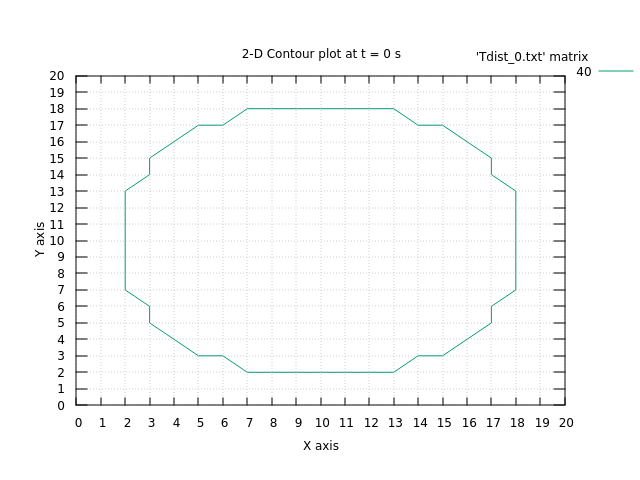
\includegraphics[width=6cm]{Tdist_0.png}}
    \subfloat{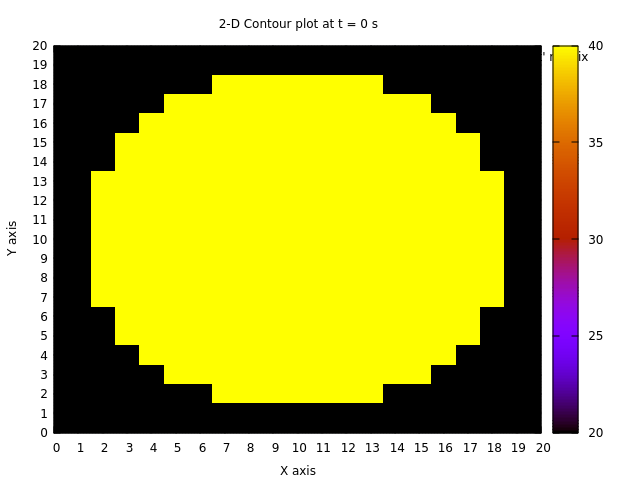
\includegraphics[width=6cm]{Tdist_0_img.png}}
    \caption{Temperature contour and image plots at t=0}
\end{figure}  

\begin{figure}[H]
    \centering
    \subfloat{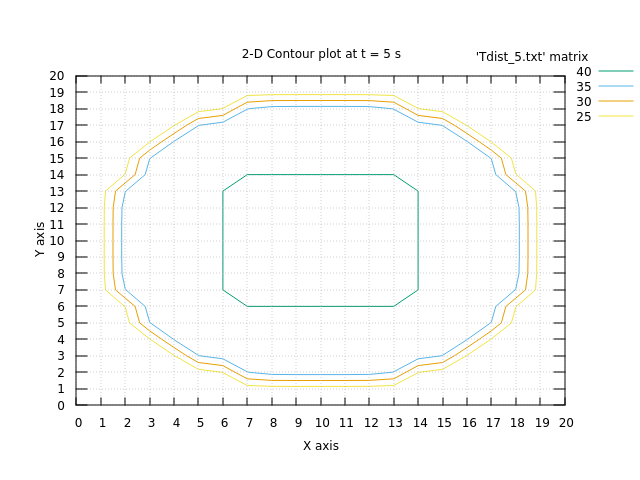
\includegraphics[width=6cm]{Tdist_5.png}}
    \subfloat{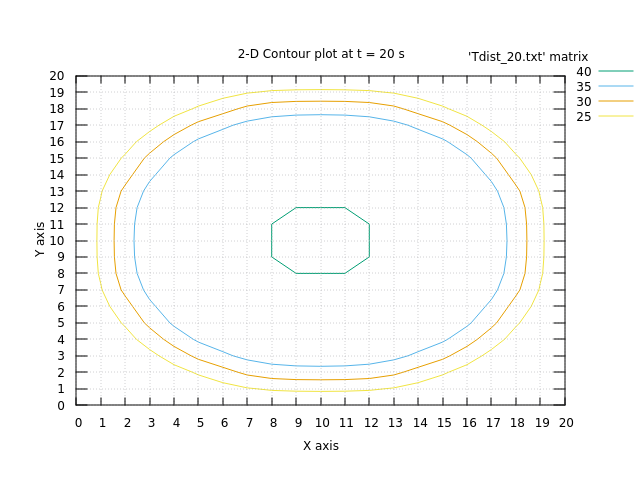
\includegraphics[width=6cm]{Tdist_20.png}}
	\vspace{-0.5cm}
    \centering
    \subfloat{{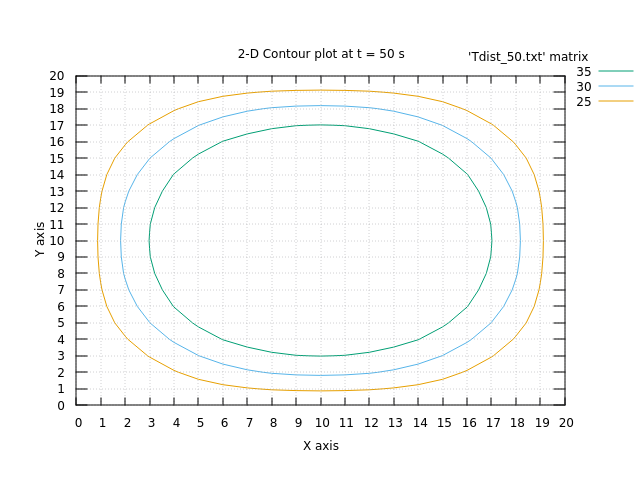
\includegraphics[width=6cm]{Tdist_50.png} }}
    \subfloat{{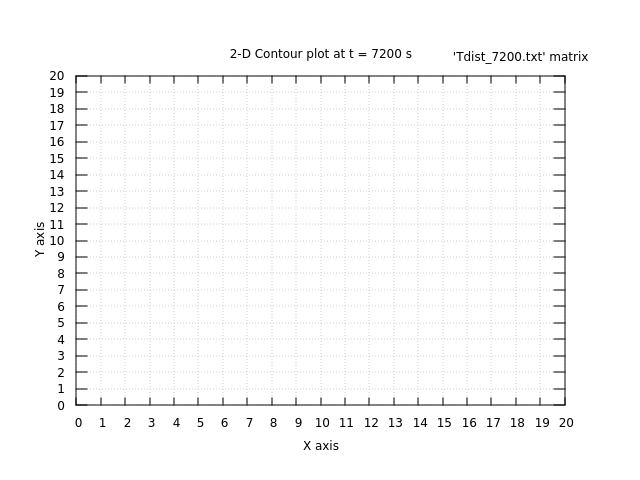
\includegraphics[width=6cm]{Tdist_7200.png} }}
    \caption{Temperature contour plots}
\end{figure}

\begin{figure}[H]
    \centering
    \subfloat{{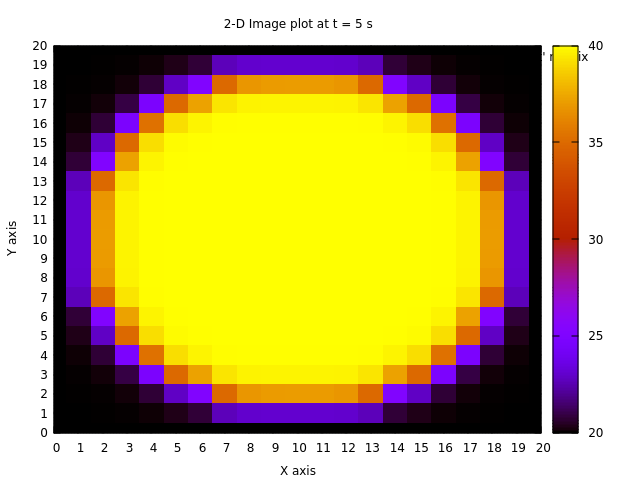
\includegraphics[width=6cm]{Tdist_5_img.png} }}
    \subfloat{{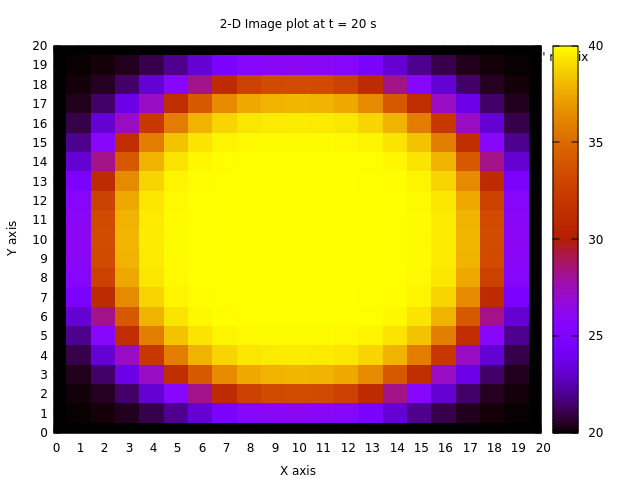
\includegraphics[width=6cm]{Tdist_20_img.png} }}
	\vspace{-0.5cm}
    \centering
    \subfloat{{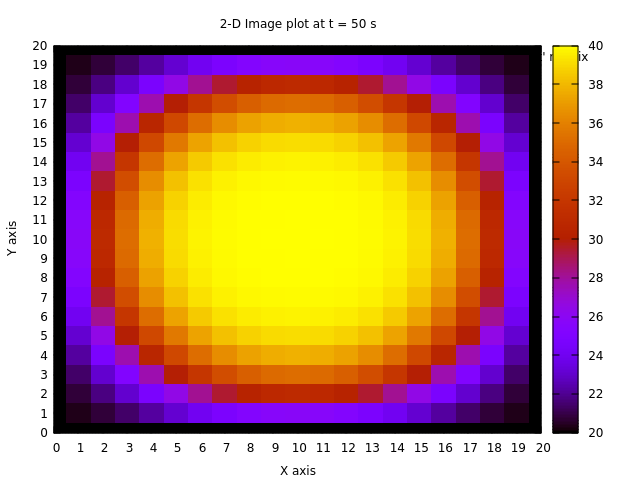
\includegraphics[width=6cm]{Tdist_50_img.png} }}
    \subfloat{{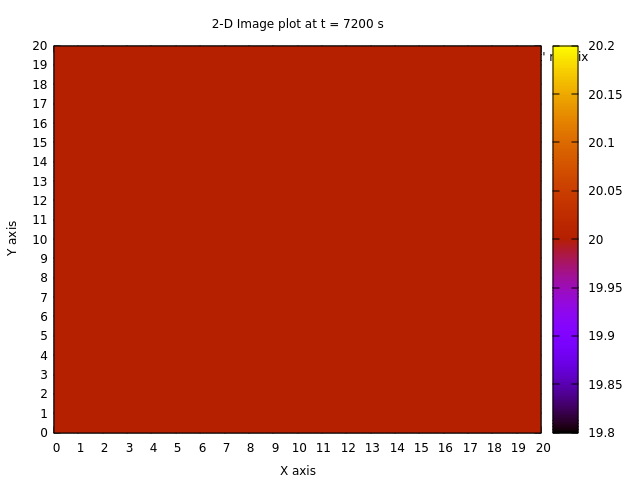
\includegraphics[width=6cm]{Tdist_7200_img.png} }}
    \caption{Temperature image plots}
\end{figure}

\emph{Note 1 : At 7200 s there is no contour plot as the plate has reached steady state condition of 20 C.}\break
\emph{Note 2 : The C++ program was compiled using gcc 7.5.0 and was run from the terminal in Ubuntu OS.}

\end{document}